\documentclass[14pt, a4paper]{extarticle}
\usepackage{GOST}
\usepackage{array}
\usepackage{verbatim}
\usepackage[detect-all]{siunitx}
\usepackage{amsmath}
\usepackage{amssymb}
\usepackage[utf8]{inputenc}
\usepackage{hyperref}

\usepackage{ifthen}

\makeatletter
\renewcommand\@biblabel[1]{#1.}
\makeatother

\usepackage{listings}
\lstset{ 
	language=python,
	basicstyle=\small\sffamily, 
	numbers=left, 
	numberstyle=\tiny,
	stepnumber=1,
	numbersep=5pt,
	showspaces=false,            
	showstringspaces=false,      
	showtabs=false,             
	frame=single,            % рисовать рамку вокруг кода
	tabsize=4,      
	commentstyle=\color{green},
	keywordstyle=\color{blue}\textbf,
	numberstyle=\scriptsize\color{gray}, % the style that is used for the line-numbers
	rulecolor=\color{black},
	captionpos=t,
	breaklines=true,         % автоматически переносить строки 
	breakatwhitespace=false, % переносить строки по пробелу
	escapeinside={\#*}{*)} 
}


\usepackage{pgfplots}
\usepackage{filecontents}
\usetikzlibrary{datavisualization}
\usetikzlibrary{datavisualization.formats.functions}

\begin{document}
	
\begin{table}[ht]
	\centering
	\begin{tabular}{|c|p{400pt}|} 
		\hline
		\begin{tabular}[c]{@{}c@{}} 
\includegraphics[scale=1]{source/b_logo.jpg} \\\end{tabular} &
		\footnotesize\begin{tabular}[c]{@{}c@{}}\textbf{Министерство~науки~и~высшего~образования~Российской~Федерации}\\\textbf{Федеральное~государственное~бюджетное~образовательное~учреждение}\\\textbf{~высшего~образования}\\\textbf{«Московский~государственный~технический~университет}\\\textbf{имени~Н.Э.~Баумана}\\\textbf{(национальный~исследовательский~университет)»}\\\textbf{(МГТУ~им.~Н.Э.~Баумана)}\\\end{tabular}  \\
		\hline
	\end{tabular}
\end{table}
\noindent\rule{\textwidth}{4pt}
\noindent\rule[14pt]{\textwidth}{1pt}
\hfill 
\noindent
\makebox{ФАКУЛЬТЕТ~}%
\makebox[\textwidth][l]{\underline{~«Информатика и системы управления»~~~~~~~~~~~~~~~~~~~~~~~~~~~~~~~~~}}%
\\
\noindent
\makebox{КАФЕДРА~}%
\makebox[\textwidth][l]{\underline{~«Программное обеспечение ЭВМ и информационные технологии»~}}%
\\

\begin{center}
	\vspace{1.5cm}
	{\bf\huge Отчёт\par}
	{\bf\Large по лабораторной работе № 4\par}
	\vspace{0.7cm}
\end{center}


\noindent
\makebox{\large{\bf Название:}~~~}
\makebox[\textwidth][l]{\large\underline{~Параллельное умножение матриц~}}\\

\noindent
\makebox{\large{\bf Дисциплина:}~~~}
\makebox[\textwidth][l]{\large\underline{~Анализ алгоритмов~~~~~~~~~~~~~~~~~~~~~~~~~~}}\\

\vspace{1.5cm}
\noindent
\begin{tabular}{l c c c c c}
	Студент      & ~ИУ7-55Б~               & \hspace{2.5cm} & \hspace{2cm}                 & &  Д.О. Склифасовский \\\cline{2-2}\cline{4-4} \cline{6-6} 
	\hspace{3cm} & {\footnotesize(Группа)} &                & {\footnotesize(Подпись, дата)} & & {\footnotesize(И.О. Фамилия)}
\end{tabular}

\noindent
\begin{tabular}{l c c c c}
	Преподователь & \hspace{5cm}   & \hspace{2cm}                 & & ~~~~~~Л.Л. Волкова~~~~~~\\\cline{3-3} \cline{5-5} 
	\hspace{3cm}  &                & {\footnotesize(Подпись, дата)} & & {\footnotesize(И.О. Фамилия)}
\end{tabular}

\vspace{0.6cm}
\begin{center}	
	\vfill
	\large \textit {Москва, 2020}
\end{center}

\thispagestyle {empty}
\pagebreak

% СОДЕРЖАНИЕ 
\clearpage
\tableofcontents

% ВВЕДЕНИЕ
\clearpage
\section*{Введение}
\addcontentsline{toc}{section}{Введение}
Цель работы: изучение возможности параллельных вычислений и использование такого подхода на практике.\par
В ходе лабораторной работы требуется:
\begin{enumerate}
	\item[1)] выбрать алгоритм для рассмотрения;
	\item[2)] описать обычную версию;
	\item[3)] выполнить 2 параллельные версии;
	\item[4)] запустить эксперименты на каждый при различном числе потоков 1,2,4,8 ...4M, где M - количество логических ядер на компьютере;
	\item[5)] проверить, всегда ли при росте потоков, время работы снижается;
	\item[6)] описать главный и рабочий поток схемой;
	\item[7)] описать точки сборки.
\end{enumerate}
В данной лабораторной работе был выбран алгоритм Винограда. Необходимо сравнить зависимость времени работы алгоритма от числа параллельных потоков и размера матриц, провести сравнение стандартного и параллельного алгоритмов.

% АНАЛИТИЧЕСКИЙ РАЗДЕЛ
\clearpage
\section{Аналитический раздел}
В данном разделе представлено описание стандартного и параллельного алгоритмов Винограда.
\subsection{Общие сведения}
Матрица — математический объект, записываемый в виде прямоугольной таблицы элементов кольца или поля (например, целых, действительных или комплексных чисел), которая представляет собой совокупность строк и столбцов, на пересечении которых находятся её элементы. Количество строк и столбцов задает размер матрицы. Хотя исторически рассматривались, например, треугольные матрицы, в настоящее время говорят исключительно о матрицах прямоугольной формы, так как они являются наиболее удобными и общими. \par
Умножение матриц — одна из основных операций над матрицами. Матрица, получаемая в результате операции умножения, называется произведением матриц.
\subsection{Алгоритм Винограда}
Если посмотреть на результат умножения двух матриц, то видно, что каждый элемент в нем представляет собой скалярное произведение соответствующих строки и столбца исходных матриц. Можно заметить также, что такое умножение допускает предварительную обработку, позволяющую часть работы выполнить заранее. \hyperref[literature]{[1]}\par
Рассмотрим два вектора $V = (v_{1},v_{2},v_{3},v_{4})$ и $W = (w_{1},w_{2},w_{3},w_{4})$. Их скалярное произведение равно:
\begin{equation}
	V * W = v_{1}w_{1} + v_{2}w_{2} + v_{3}w_{3} + v_{4}w_{4}
\end{equation}
Это равенство можно переписать в виде:
\begin{equation}
	V * W = (v_{1} + w_{2})(v_{2} + w_{1}) + (v_{3} + w_{4})(v_{4} + w_{3}) -  v_{1}v_{2} - v_{3}v_{4} - w_{1}w_{2} - w_{3}w_{4}
\end{equation}
Менее очевидно, что выражение в правой части последнего равенства допускает предварительную обработку: его части можно вычислить заранее и запомнить для каждой строки первой матрицы и для каждого столбца второй. На практике это означает, что над предварительно обработанными элементами придется выполнять лишь первые два умножения и последующие пять сложений, а также дополнительно два сложения. 
\subsection{Параллельное программирование}
Параллельное программирование. Параллельное программирование служит для создания программ, эффективно использующих вычислительные ресурсы за счет одновременного исполнения кода на нескольких вычислительных узлах. Для создания параллельных приложений используются параллельные языки программирования и специализированные системы поддержки параллельного программирования, такие как MPI и OpenMP. Параллельное программирование является более сложным по сравнению с последовательным как в написании кода, так и в его отладки. Для облегчения процесса параллельного программирования существуют специализированные инструменты, например, отладчик TotalView.\hyperref[literature]{[2]}
\subsection{Параллельный алгоритм Винограда}
Для того, чтобы добиться большей эффективности алгоритма умножения матриц Винограда, необходимо расспараллелить ту часть алгоритма, которая содержит больше всего вложенных циклов. Вычисление результата для каждой строки не зависит от результата умножения для других строк. Каждый поток будет выполнять вычисления определенных строк результирующей матрицы.\par
Для проверки эффективности выбранного метода, также можно распаралелить циклы двойной вложенности в начале алгоритма (циклы вычисления векторов mulH и mulV).
\subsection{Вывод}
Было представлено математическое описание стандартного и параллельного алгоритмов Винограда. Основная идея заключается в том, чтобы распараллелить главный цикл тройной вложенности.

\clearpage
\section{Конструкторский раздел}
В данном разделе представлены схемы разработанных алгоритмов. Также описывается часть алгоритма, которая будет распараллеливаться.
\subsection{Разработка алгоритма}
На \hyperref[Algorithm1]{рисунке 1} изображена схема стандартного алгоритма умножения матриц.
\begin{figure}[h!]\label{Algorithm1}
	\center{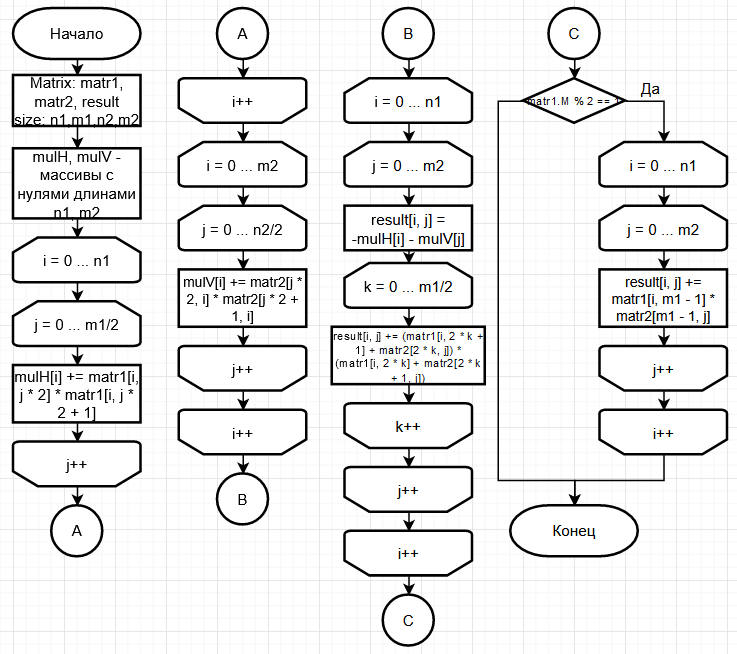
\includegraphics[scale=0.8]{source/Algorithm.png}}
	\caption{Схема стандартного алгоритма умножения матриц}
\end{figure}
\subsection{Распараллеливание программы}
В представленном алгоритме будет распараллеливаться цикл тройной вложенности (участок между B и C). Это должно ускорить время работы алгоритма.\par
Также для проверки эффективности будут распараллеливаться два первых цикла отдельно. Будут построены графики для данной реализации и сравниться время работы алгоритмов.
\subsection{Вывод}
В данном разделе была рассмотрена схема алгоритма Винограда и описалась часть алгоритма, которая будет распараллеливаться.

\clearpage
\section{Технологический раздел}
В данном разделе даны общие требования к программе, средства реализации и сама реализация алгоритмов.



\clearpage
\section*{Литература}
\addcontentsline{toc}{section}{Литература}
\begin{enumerate}
	\label{literature}
	\item Умножение матриц. -URL: \href{http://www.algolib.narod.ru/Math/Matrix.html}{http://www.algolib.narod.ru/Math/Matrix.html} (дата обращения: 24.10.2020). -Текст: электронный.
	\item Параллельное программирование. -URL: \href{https://www.viva64.com/ru/t/0038/}{https://www.viva64.com/ru/t/0038/} (дата обращения: 24.10.2020). -Текст: электронный.
	\item  Документация по C\#. -URL: \href{https://docs.microsoft.com/ru-ru/dotnet/csharp/}{https://docs.microsoft.com/ru-ru/dotnet/csharp/} (дата обращения: 24.10.2020). -Текст: электронный.
	\item Документация по семейству продуктов Visual Studio. -URL:\par \href{https://docs.microsoft.com/ru-ru/visualstudio/?view=vs-2019}{https://docs.microsoft.com/ru-ru/visualstudio/?view=vs-2019 } (дата обращения: 01.10.2020). -Текст: электронный.
	\item Stopwatch Класс. -URL: \href{https://goo.su/2e99}{https://goo.su/2e99 } (дата обращения: 24.10.2020). -Текст: электронный.
	\item Под капотом у Stopwatch. -URL:  \href{https://habr.com/ru/post/226279/}{https://habr.com/ru/post/226279/} (дата обращения: 24.10.2020). Текст: электронный.
\end{enumerate}
\end{document}\par